\section{Результаты работы четвертой лабораторной работы}

\subsection{Задание}

1. Дата отчета: 29 апреля

2. 4 работа начинается на неделю позже

3. 10 задача на 80 процентов выполнена

4. 6 работа закончилась на неделю позже

5. С 1 апреля системный аналитик занят в другом проекте и здесь работает только на 50 процентов

6. С 10 апреля увеличивается аренда сервера

7. С 10 апреля программист 3 заболел на неделю

8. С 15 марта ведущий программист на повышение квалификации на 10 процентов увеличивается зарплата

\subsection{Дата отчета}

\begin{figure}[ht!]
	
\includegraphics[width=0.75\linewidth]{assets/images/Screenshot 2024-03-09 at 11.26.27.png}
	\label{fig:r2}
	\caption{Сдвиг проекта}
\end{figure}
\FloatBarrier

\begin{figure}[ht!]
	
\includegraphics[width=0.75\linewidth]{assets/images/Screenshot 2024-03-09 at 11.27.40.png}
	\label{fig:r2}
	\caption{4 Задача сдвинута}
\end{figure}
\FloatBarrier

Сроки сдвинулись на неделю.


\begin{figure}[ht!]
	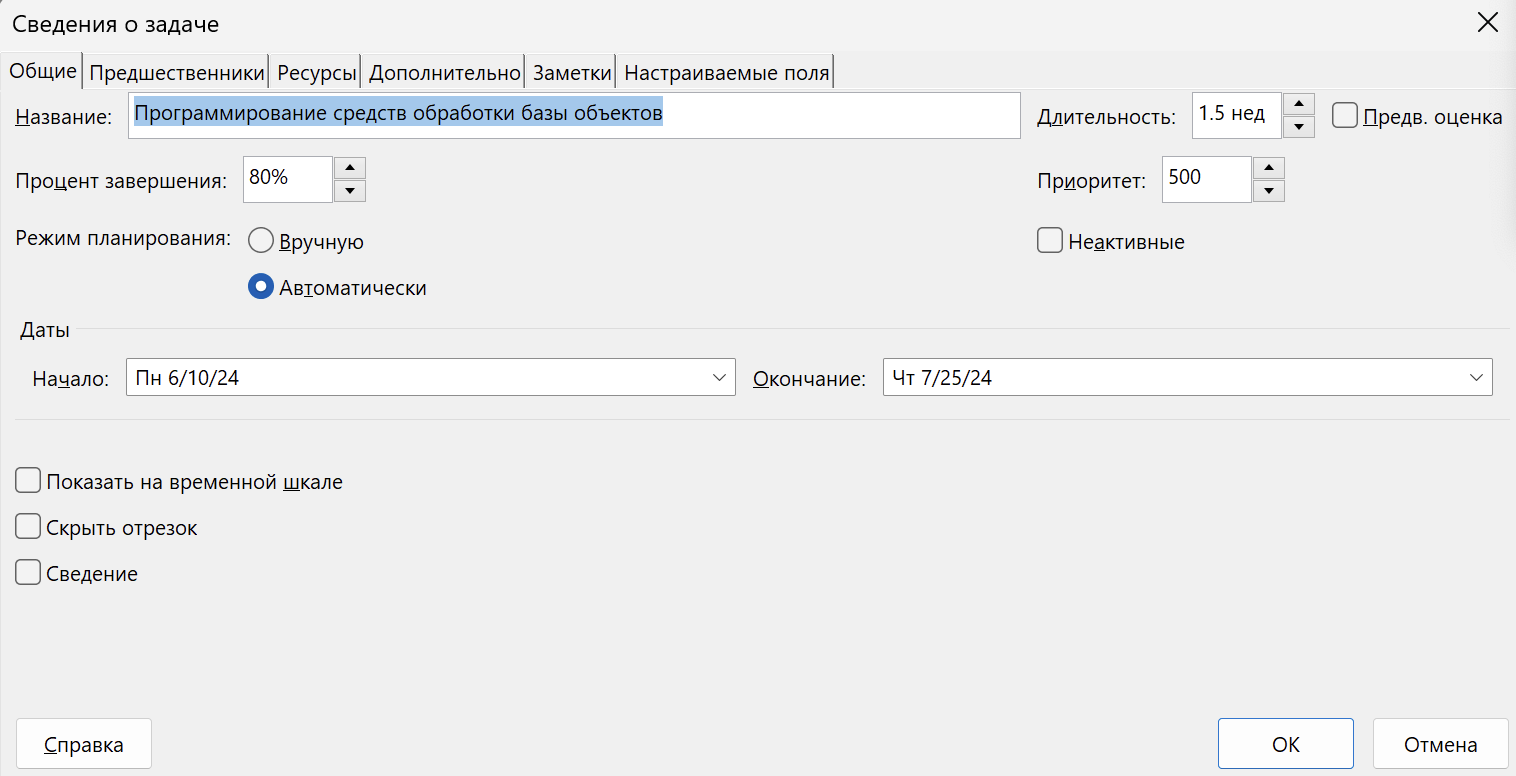
\includegraphics[width=0.75\linewidth]{assets/images/Screenshot 2024-03-09 at 11.28.59.png}
	\label{fig:r2}
	\caption{10 Задача выполнена на 80 процентов}
\end{figure}
\FloatBarrier

Сроки сдвинулись на два дня назад.

\begin{figure}[ht!]
	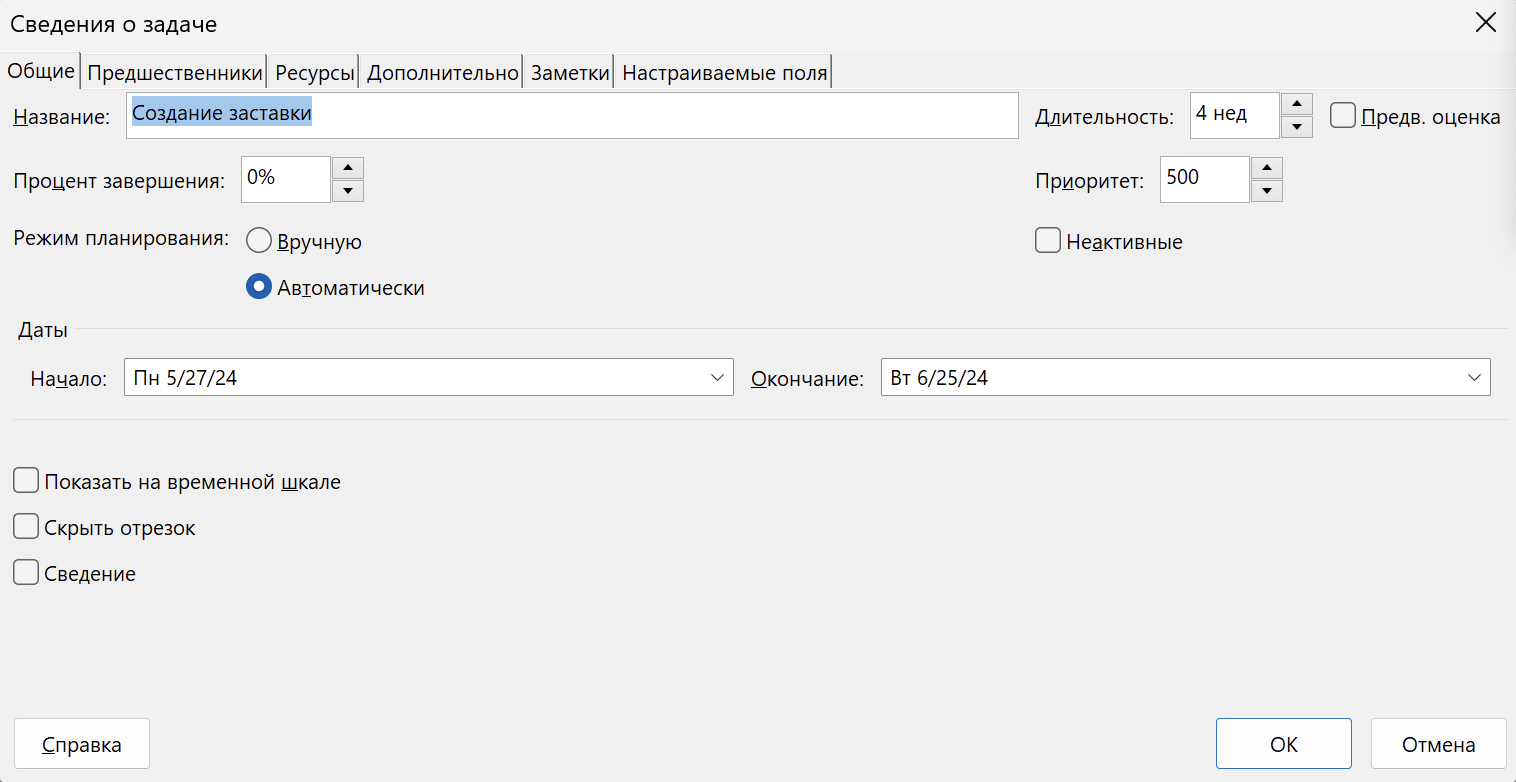
\includegraphics[width=0.75\linewidth]{assets/images/Screenshot 2024-03-09 at 11.30.35.png}
	\label{fig:r2}
	\caption{На неделю сдвинута 6 задача}
\end{figure}
\FloatBarrier

\begin{figure}[ht!]
	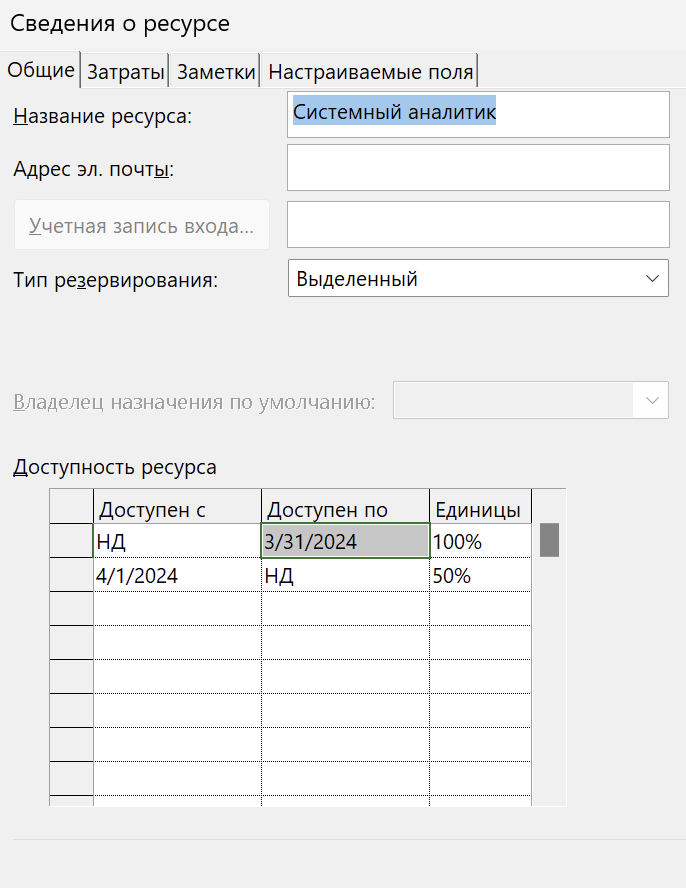
\includegraphics[width=0.75\linewidth]{assets/images/Screenshot 2024-03-09 at 11.31.44.png}
	\label{fig:r2}
	\caption{С 1 апреля системный аналитик занят в другом проекте и здесь работает только на 50 процентов}
\end{figure}
\FloatBarrier

сроки сдвинулись на две недели

\begin{figure}[ht!]
	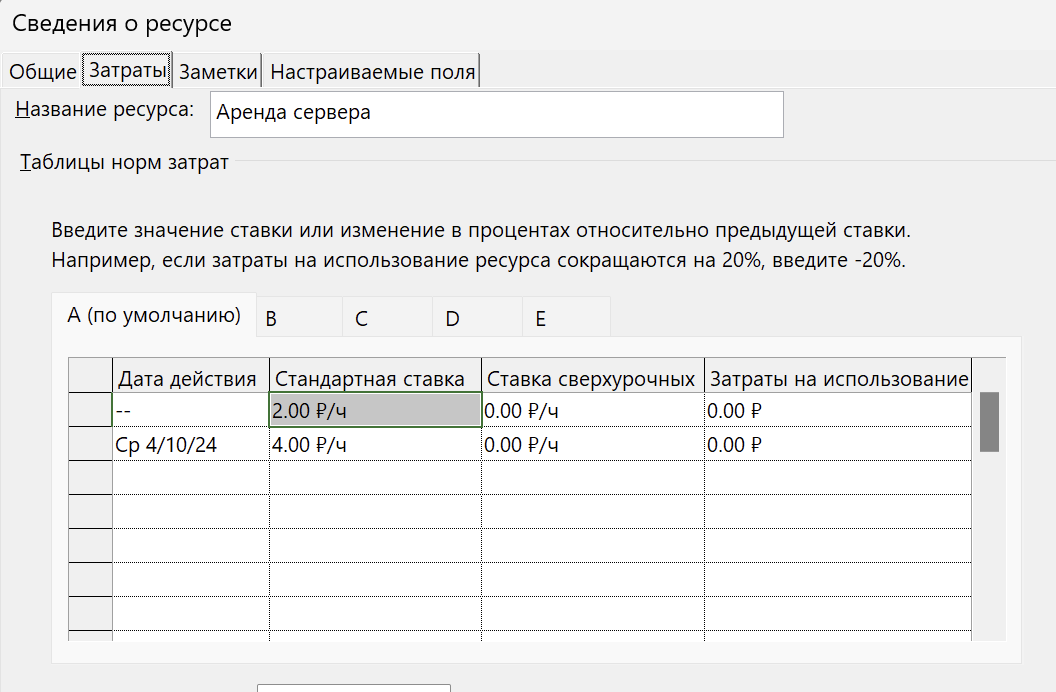
\includegraphics[width=0.75\linewidth]{assets/images/Screenshot 2024-03-09 at 11.32.38.png}
	\label{fig:r2}
	\caption{С 10 апреля увеличивается аренда сервера в два раза}
\end{figure}
\FloatBarrier


\begin{figure}[ht!]
	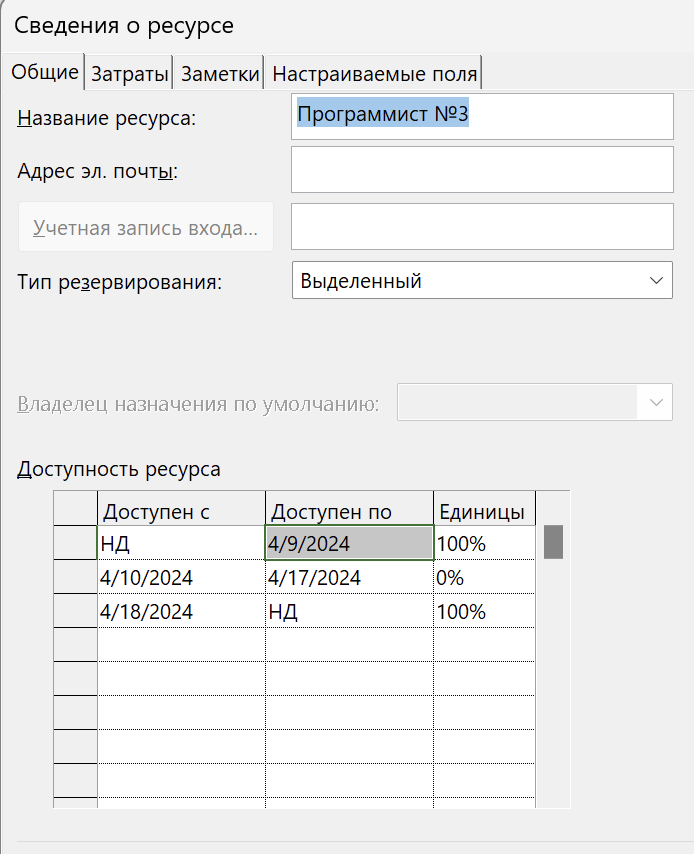
\includegraphics[width=0.75\linewidth]{assets/images/Screenshot 2024-03-09 at 11.34.40.png}
	\label{fig:r2}
	\caption{С 10 апреля программист 3 заболел на неделю}
\end{figure}
\FloatBarrier

\begin{figure}[ht!]
	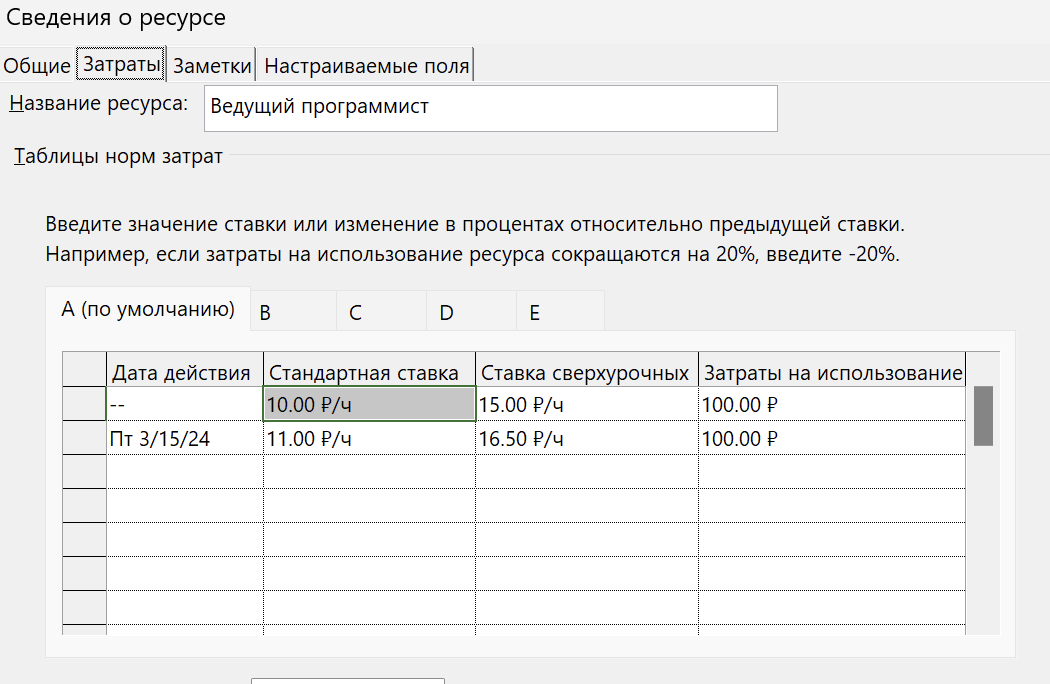
\includegraphics[width=0.75\linewidth]{assets/images/Screenshot 2024-03-09 at 11.35.29.png}
	\label{fig:r2}
	\caption{С 15 марта ведущий программист на повышение квалификации на 10 процентов увеличивается зарплата}
\end{figure}
\FloatBarrier


Возникли перегрузки и они были выравнены с такими параметрами

\begin{figure}[ht!]
	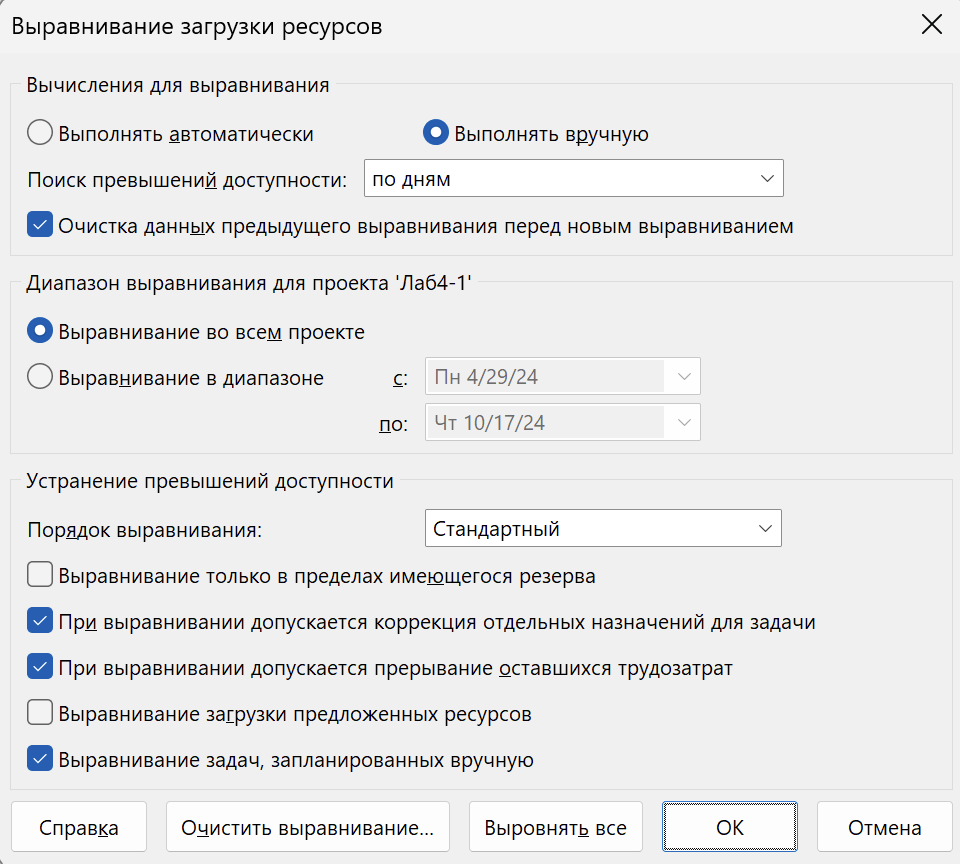
\includegraphics[width=0.75\linewidth]{assets/images/Screenshot 2024-03-09 at 11.37.19.png}
	\label{fig:r2}
	\caption{Выравнивание}
\end{figure}
\FloatBarrier

Проект стал заканчиваться 29.08, а бюджет возрос до 49011.74 рублей.

\begin{figure}[ht!]
	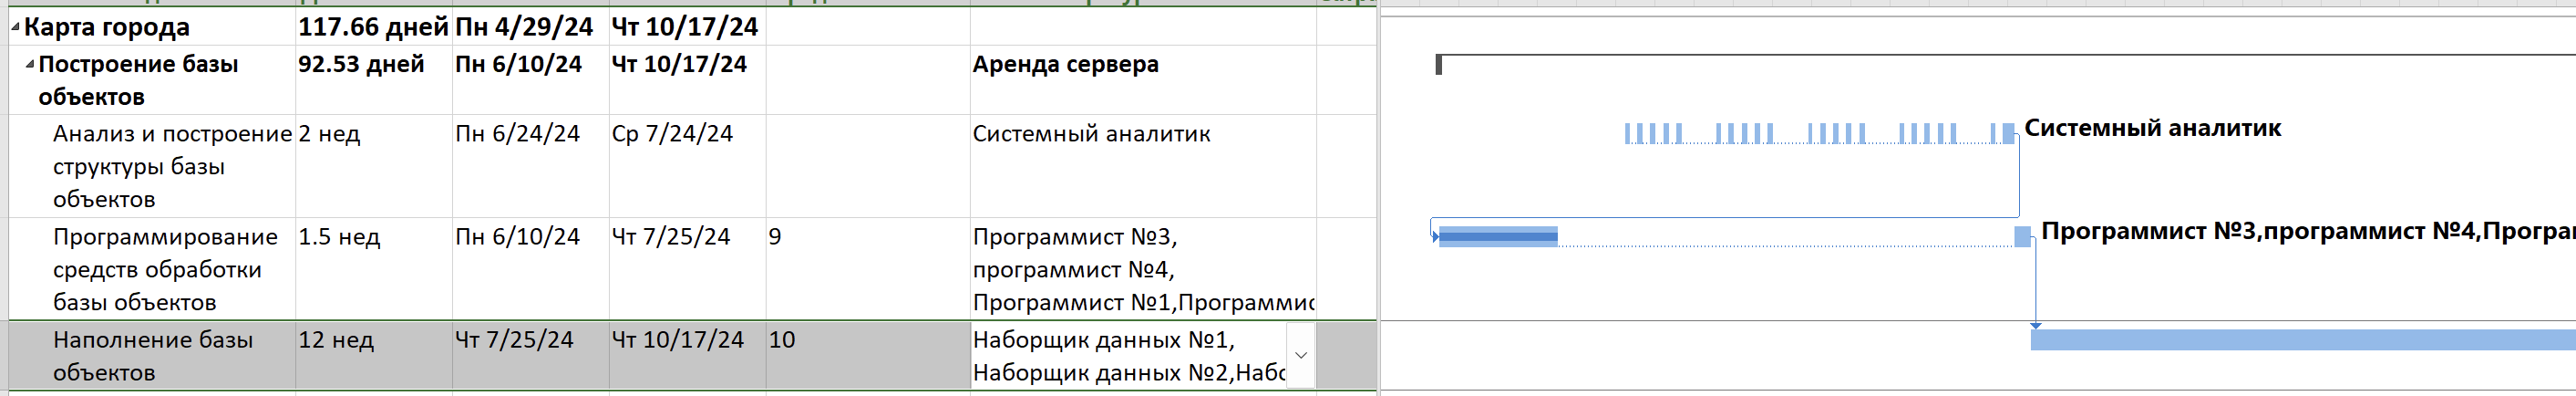
\includegraphics[width=0.75\linewidth]{assets/images/Screenshot 2024-03-09 at 11.39.55.png}
	\label{fig:r2}
	\caption{Критические задачи}
\end{figure}
\FloatBarrier

Остались три критические задачи, для них нет свободных дополнительных рессурсов.
Можно решить наймом дополнительных рессурсов.


Таким образом, соотношение трудозатрат к затратам практически не изменилось. Увеличились затраты на программистов (около 3).

За счет фиксированных трудовых рессурсов, при назначании программистов на задачи, было сокращено время задач.


За счет выполенения 10 задачи на 80 процентов вместо 49 процентов. Бюджет проект удалось сократить до 47583.06 рублей

\subsection*{Вывод}

В результате лабораторной работы были отработаны навыки использования программы Microsoft Project для оптимизации временных и финансовых показателей проекта. 
Итак, затраты составляют 47583.06 руб. (было 48 076,67), что находится в рамках выделенного бюджета, дата окончания проекта –-- 29.08.2022 (была 22.07.2022).
